\documentclass[a4paper]{article}
\usepackage{lmodern}
\usepackage{amssymb,amsmath}
\usepackage{ifxetex,ifluatex}
\usepackage{fixltx2e} % provides \textsubscript
\ifnum 0\ifxetex 1\fi\ifluatex 1\fi=0 % if pdftex
  \usepackage[T1]{fontenc}
  \usepackage[utf8]{inputenc}
\else % if luatex or xelatex
  \ifxetex
    \usepackage{mathspec}
  \else
    \usepackage{fontspec}
  \fi
  \defaultfontfeatures{Ligatures=TeX,Scale=MatchLowercase}
\fi
% use upquote if available, for straight quotes in verbatim environments
\IfFileExists{upquote.sty}{\usepackage{upquote}}{}
% use microtype if available
\IfFileExists{microtype.sty}{%
\usepackage{microtype}
\UseMicrotypeSet[protrusion]{basicmath} % disable protrusion for tt fonts
}{}
\usepackage[margin=1in]{geometry}
\usepackage{hyperref}
\hypersetup{unicode=true,
            pdftitle={Minimizing Programming Assignment Plagiarism},
            pdfauthor={Sridhar Adhikarla (sriad858)},
            pdfborder={0 0 0},
            breaklinks=true}
\urlstyle{same}  % don't use monospace font for urls
\usepackage{graphicx,grffile}
\makeatletter
\def\maxwidth{\ifdim\Gin@nat@width>\linewidth\linewidth\else\Gin@nat@width\fi}
\def\maxheight{\ifdim\Gin@nat@height>\textheight\textheight\else\Gin@nat@height\fi}
\makeatother
% Scale images if necessary, so that they will not overflow the page
% margins by default, and it is still possible to overwrite the defaults
% using explicit options in \includegraphics[width, height, ...]{}
\setkeys{Gin}{width=\maxwidth,height=\maxheight,keepaspectratio}
\IfFileExists{parskip.sty}{%
\usepackage{parskip}
}{% else
\setlength{\parindent}{0pt}
\setlength{\parskip}{6pt plus 2pt minus 1pt}
}
\setlength{\emergencystretch}{3em}  % prevent overfull lines
\providecommand{\tightlist}{%
  \setlength{\itemsep}{0pt}\setlength{\parskip}{0pt}}
\setcounter{secnumdepth}{0}
% Redefines (sub)paragraphs to behave more like sections
\ifx\paragraph\undefined\else
\let\oldparagraph\paragraph
\renewcommand{\paragraph}[1]{\oldparagraph{#1}\mbox{}}
\fi
\ifx\subparagraph\undefined\else
\let\oldsubparagraph\subparagraph
\renewcommand{\subparagraph}[1]{\oldsubparagraph{#1}\mbox{}}
\fi

%%% Use protect on footnotes to avoid problems with footnotes in titles
\let\rmarkdownfootnote\footnote%
\def\footnote{\protect\rmarkdownfootnote}

%%% Change title format to be more compact
\usepackage{titling}

% Create subtitle command for use in maketitle
\newcommand{\subtitle}[1]{
  \posttitle{
    \begin{center}\large#1\end{center}
    }
}

\setlength{\droptitle}{-2em}

  \title{Minimizing Programming Assignment Plagiarism}
    \pretitle{\vspace{\droptitle}\centering\huge}
  \posttitle{\par}
    \author{Sridhar Adhikarla (sriad858)}
    \preauthor{\centering\large\emph}
  \postauthor{\par}
      \predate{\centering\large\emph}
  \postdate{\par}
    \date{September 28, 2018}


\begin{document}
\maketitle

\subsection{Abstract}\label{abstract}

Technology helps students develop but it also attracts plagiarism.
Availability of electronic material through the internet has a great
positive impact on students, they get to learn a lot, and on the
downside also increases the risk of intentional or unintentional
plagiarism among students. Plagiarism is not just confined to an essay
or text-based assignments. Programming assignments, being a part of most
computer-based courses, have a different kind of plagiarism and it is
difficult to detect. This paper explores the different reasons leading
to plagiarism in programming assignments and examines ways we can detect
and minimize it.

\subsection{Introduction}\label{introduction}

In today's world, we can get any information we want, be it medical
diagnosis or directions to go somewhere, over the internet. Same is the
case with programming assignments, students can get all the source code
for the assignment over the internet, creating a risk of intentional or
unintentional plagiarism. The internet can be a great source of
knowledge for the ones who look for it, but if someone just copies the
source code for the assignment over the internet, they are not learning
anything from it and are failing the sole purpose of the assigned task.
Plagiarism in programming assignments is one of the most common things
in computer-based courses, and it is increasing every year. Although it
is not clear if the increase is due to the improved algorithm for
plagiarism checking or more number of students involving in plagiarism.
Students should know the value and purpose of the task assigned to them,
and they should also be aware of how to prevent themselves from
plagiarism. This is the reason teachers should create awareness not just
about plagiarism in text-based assignments but also for programming
assignments. Students should be taught what is right and what is wrong.

Plagiarism in programming assignments is different from the text-based
assignments, and there is no common definition for source-code
plagiarism. According to Faidhi and Robinson (2010), ``plagiarism occurs
when programming assignments are copied and transformed with very little
effort from the students'', whereas Joy and Luck (2010) define
plagiarism as, ``unacknowledged copying of documents and programs''. A
lot of institutions use text similarity-based plagiarism detection tools
for programming assignments, which is not an effective way to do it. The
lexical elements of the code can be modified while retaining the
structure and logic of copied source code, and a text similarity
plagiarism detector cannot detect that. In this paper we will talk
about, how much do students know about source code plagiarism and some
of the softwares for source code plagiarism detection.

\subsection{Student's knowledge about plagiarism in
programming}\label{students-knowledge-about-plagiarism-in-programming}

There has been a lot of research on how to improve plagiarism detectors
in the past few years and very few answering the main problem causing
it, “Do the student know what constitutes as plagiarism?”, Paul
Clough (2000). It is very important for the students to have a clear
idea of what is right and what is wrong. Most institutions focus on
teaching students about plagiarism in text-based assignments and not
about plagiarism in programming code. The definition of plagiarism is
very different between the two. If the institutions start focusing on
teaching the students, the correct ways to avoid plagiarism in
programming assignments this would reduce a lot of unintentional
plagiarism.

In the paper, “Source code plagiarism- A student’s perspective”
(2010), the authors, conducted a survey for students from computer
background all over UK and Europe, to find out how much students knew
about Plagiarism in Programming. There were 15 questions in the survey
and for every right answer the student got +1 points and for every wrong
answer, the student got -1. The total number of students who
participated in the survey was 770, of which 615 were from UK and 87
from Europe and the remaining from the rest of the world. The mean score
obtained by students in Europe and UK was just 7.6 out of 15. Figure-1
gives us a clear idea that students lack knowledge in the field, or
there is some confusion in them about what is plagiarism. The frequency
plot for the scores obtained by the students shows clearly that only a
few have a clear idea about the subject of source code plagiarism.

\begin{figure}
\centering
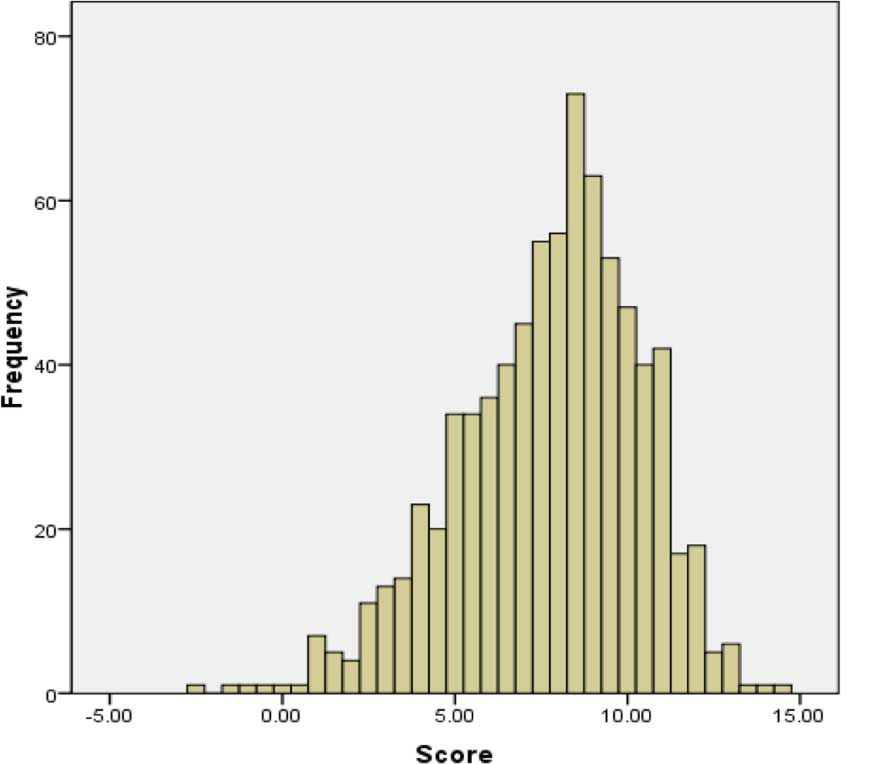
\includegraphics[width=3.12500in]{plotAAS.png}
\caption{Students score frequency plot}
\end{figure}

The findings give a clear message that, along with detection and
enforcement of appropriate penalties, it is also necessary to look
beyond to understand clearly why plagiarism is so widespread. This study
gives us a clear idea that for students writing program code, the
training given is not effective in raising awareness of what constitutes
plagiarism. Some areas of confusion in student’s mind are debatable,
such as self-plagiarism and different definitions of plagiarism between
institutions.

\subsection{Plagiarism detection in programming
languages}\label{plagiarism-detection-in-programming-languages}

Automated methods for finding plagiarism in student’s source code
submissions have been in use for a very long time and there are many
available search engines and services for it. The most common and
effective technique for plagiarism detection in the source code is
tokenizing the code and then searching a pair of submissions for long
common substrings. According to Thomas Lancaster (2004), some of the
widely used services, that use this technique for plagiarism detection
in the source code, are MOSS and JPlag. These are the services that are
used by a majority of the institutions for detecting source code
plagiarism in student submissions. Although this detection is well
established, future research for improving these are going on and a lot
of extensions have been made for these methods to improve results.
PlaGate, as described by Mike Joy and Georgina Cosma (2011), is one such
extension created. It is a novel tool that can be integrated into the
existing detection tool to improve the performance. PlaGate implements a
new approach for investigating the similarities between source code with
a view to gathering evidence for proving plagiarism.

MOSS (Measure of Software Similarity), developed in 1994, as described
in a paper by Sun Zhigang (2012) is an automatic system for detecting
the similarity of programs. MOSS was created for detecting similarities
between software’s, but to date, the main application of MOSS is
detecting plagiarism in programming classes at institutions. The input
to MOSS is a set of programs, and it returns references, the teacher
must manually check through the references to confirm who is cheating.
The only weakness of MOSS is that it does not do a web search, but this
is not a big problem as it common that for a large class, more than one
student copies code from the same source. MOSS can easily catch such
similarities. On using extensions like PlaGate with MOSS we will get
exact results for students involved in cheating with evidence.

JPlag, described in a paper by Lutz Prechelt (2002), is another such
service for source code plagiarism detection. It is written in Java
programming language and this works only with programming languages that
are similar in syntax to Java. JPlag is mostly used for plagiarism
detection with languages like Java, C, C++. The input to JPlag is a set
of programs. It compares these programs pairwise, computing total
similarity value for each pair and a set of similarity regions. JPlag
converts each program into a string of canonical tokens. For the
comparison of two programs, JPlag then covers one such token string by
substrings taken from the other where possible.

\subsection{Conclusion}\label{conclusion}

Programming assignments are an important part of a course curriculum as
they give the practical experience to the students. It plays a key role
in shaping the learning curve of students. I think if proper knowledge
is not provided to the students about plagiarism in programming
assignments and appropriate techniques are not used for detecting
plagiarism in the source code, the students are the one who suffers.
They miss out on the most important part of the learning curve of the
course. Students should be made aware of plagiarism and its
consequences, that would motivate them to put some effort into their
assignments.

If the students are made aware of the techniques to use to avoid
plagiarism in programming and proper services, like MOSS and JPlag, are
used to detect plagiarism in programming assignments, this would reduce
plagiarism and even benefit the learning of students.

\subsubsection*{References}\label{references}
\addcontentsline{toc}{subsubsection}{References}

\hypertarget{refs}{}
\hypertarget{ref-Paul}{}
Clough, Paul. 2000. ``Plagiarism in Natural and Programming Languages:
An Overview of Current Tools and Technologies.'' \emph{Department of
Computer Science, University of Sheffield} 1 (1). CSUOS: 1--31.
\href{\%20http://citeseerx.ist.psu.edu/viewdoc/summary?doi=10.1.1.65.774}{http://citeseerx.ist.psu.edu/viewdoc/summary?doi=10.1.1.65.774}.

\hypertarget{ref-Mike_Joy_Cosma}{}
Georgina Cosma, Mike Joy. 2011. ``An Approach to Source-Code Plagiarism
Detection and Investigation Using Latent Semantic Analysis.'' \emph{IEEE
Transactions on Computers} 61 (4). IEEE: 379--94.
doi:\href{https://doi.org/12486990}{12486990}.

\hypertarget{ref-Lutz_Guido_Michal}{}
Lutz Prechelt, Michael Philippsen, Guido Malpohl. 2002. ``Finding
Plagiarisms Among a Set of Programs with Jplag.'' \emph{Universal
Computer Science} 8 (11). JUCS: 1016--38.

\hypertarget{ref-Mike_Cosma_Jane2}{}
Mike Joy, Jane Yin-Kim Yau, Georgina Cosma. 2010. ``Source Code
Plagiarism-a Student Perspective.'' \emph{IEEE Transactions on
Education} 54 (1). IEEE: 125--32.
doi:\href{https://doi.org/5451097}{5451097}.

\hypertarget{ref-Sanjay_Rao}{}
Sanjay Goel, Deepak Rao. 2010. ``Plagiarism and Its Detection in
Programming Languages.'' \emph{Technical Report, Department of Computer
Science and Information Technology, JIITU} 1 (1). JIITU: 1--8.
\href{\%20https://pdfs.semanticscholar.org/23c7/03bde13f95b2690c035cd5811fbe2c6f113e.pdf}{https://pdfs.semanticscholar.org/23c7/03bde13f95b2690c035cd5811fbe2c6f113e.pdf}.

\hypertarget{ref-Sun_su_zhu}{}
Sun Zhigang, Zhu Ning, Su Xiaohong. 2012. ``Moodle Plugins for Highly
Efficient Programming Courses.'' \emph{Moodle Research Conference} 1
(1). MRC: 157--63.
\href{\%20https://research.moodle.net/51/1/20\%20-\%20Zhigang\%20-\%20Moodle\%20Plugins\%20for\%20Highly\%20Efficient\%20Programming\%20Courses.pdf}{https://research.moodle.net/51/1/20\%20-\%20Zhigang\%20-\%20Moodle\%20Plugins\%20for\%20Highly\%20Efficient\%20Programming\%20Courses.pdf}.

\hypertarget{ref-Thomas_Fintan}{}
Thomas Lancaster, Fintan Culwin. 2004. ``A Comparison of Source Code
Plagiarism Detection Engines.'' \emph{Computer Science Education} 14
(2). CSE: 101--12.
doi:\href{https://doi.org/10.1080/07377363.2014.956027}{10.1080/07377363.2014.956027}.


\end{document}
